\chapter{Practice: Sleep}
Flash an XBee with the End-Device AT firmware using X-CTU.
First, plug the XBee in the XBee explorer socket and connect the USB cable.
Use the \texttt{dmesg} command to find to which device is the USB attached.
Look for a line similar to

\texttt{[ 6370.421000] usb 3-2.2: FTDI USB Serial Device converter now attached to ttyUSB0}

The command to invoke X-CTU will be something similar to

\texttt{wine .wine/drive\_c/Program{\textbackslash} Files/Digi/XCTU/X-CTU.exe}

Then set the port as in Fig. \ref{fig:set-port} and test that you can connect to the XBee using the ``Test/Query'' button as in Fig.~\ref{fig:test-xctu}.
\begin{figure}[htbp]
  \centering
  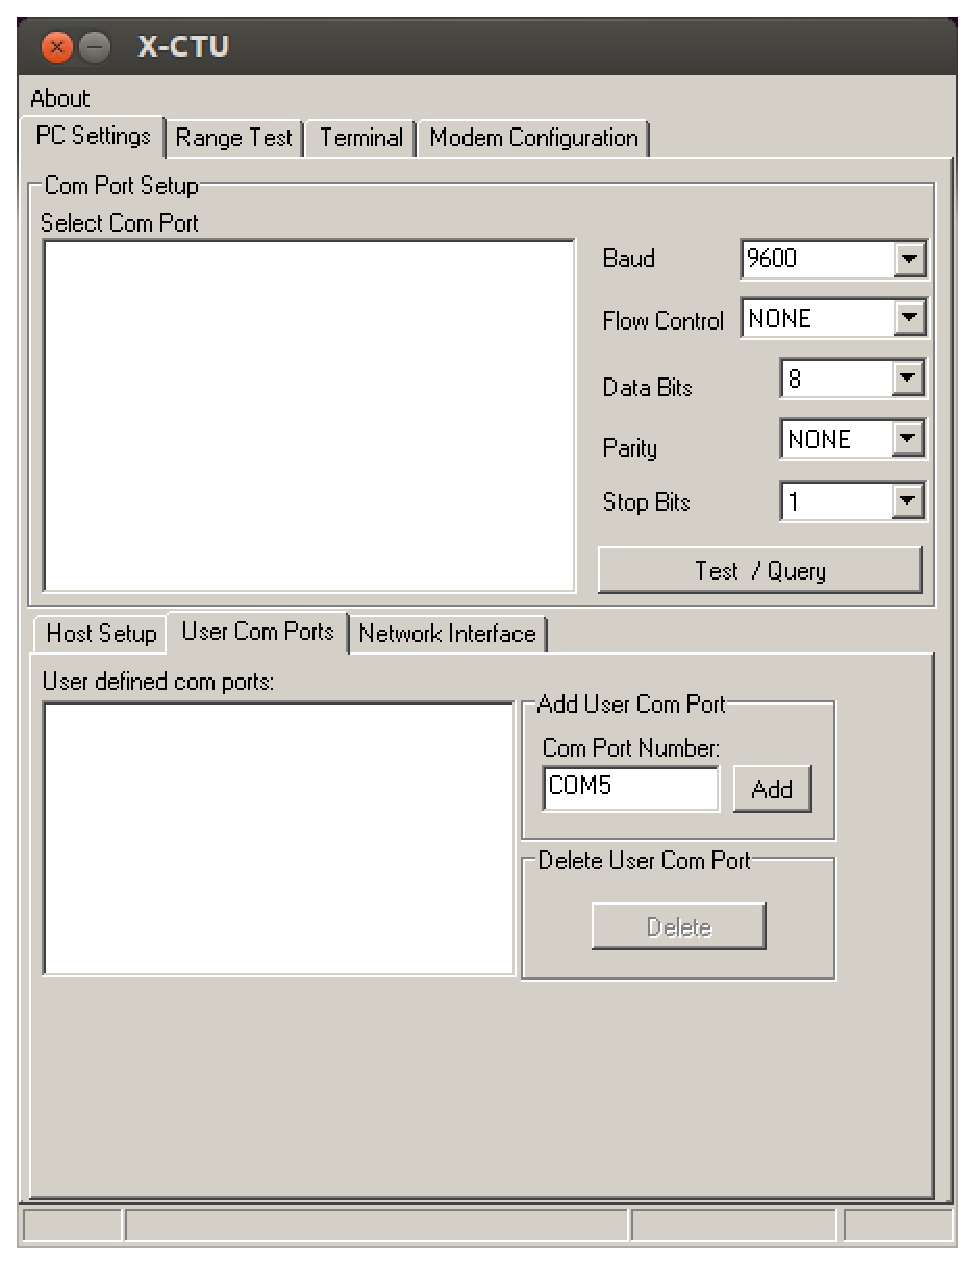
\includegraphics[width=0.3\linewidth]{figures/set-port.eps}
  \caption{Setting the port.}
  \label{fig:set-port}
\end{figure}

\begin{figure}[htbp]
  \centering
  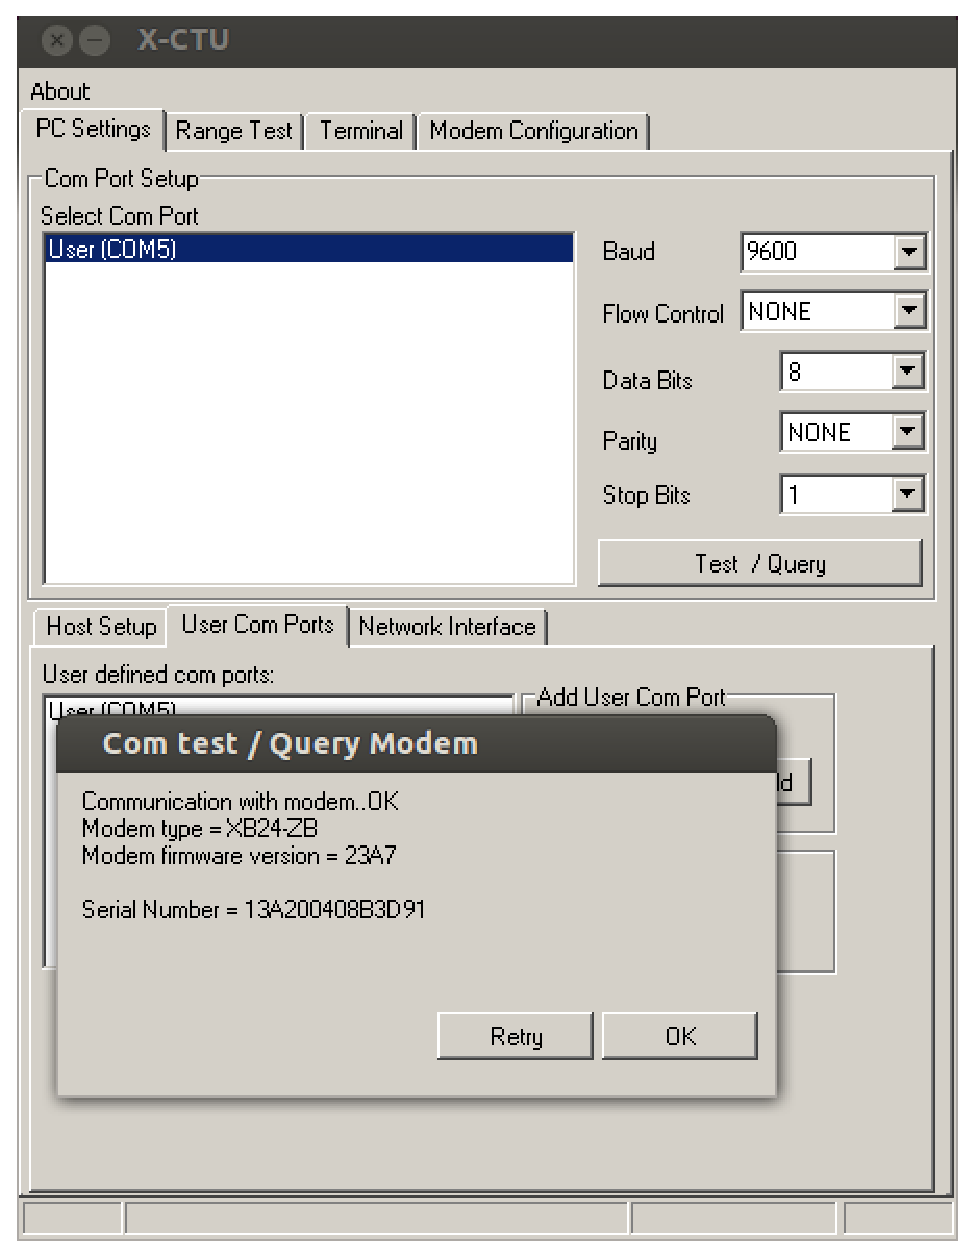
\includegraphics[width=0.3\linewidth]{figures/test-xctu.eps}
  \caption{Testing communication with the XBee.}
  \label{fig:test-xctu}
\end{figure}

Now we switch to the ``Modem Configuration'' tag.
We will flash the XBee with an ``end device'' firmware.
Only end devices can sleep.
Routers and coordinators must be always up.
We choose, for example, the firmware ``zigbee end device at'' in the ``Function set'' drop down menu.
And we write the firmware to the XBee.

Let's also clean all previous configuration.
Click the ``restore'' and ``read'' buttons to restore settings to defaults.
You should obtain something similar to Fig. \ref{fig:clean-28a7}.

\begin{figure}[htbp]
  \centering
  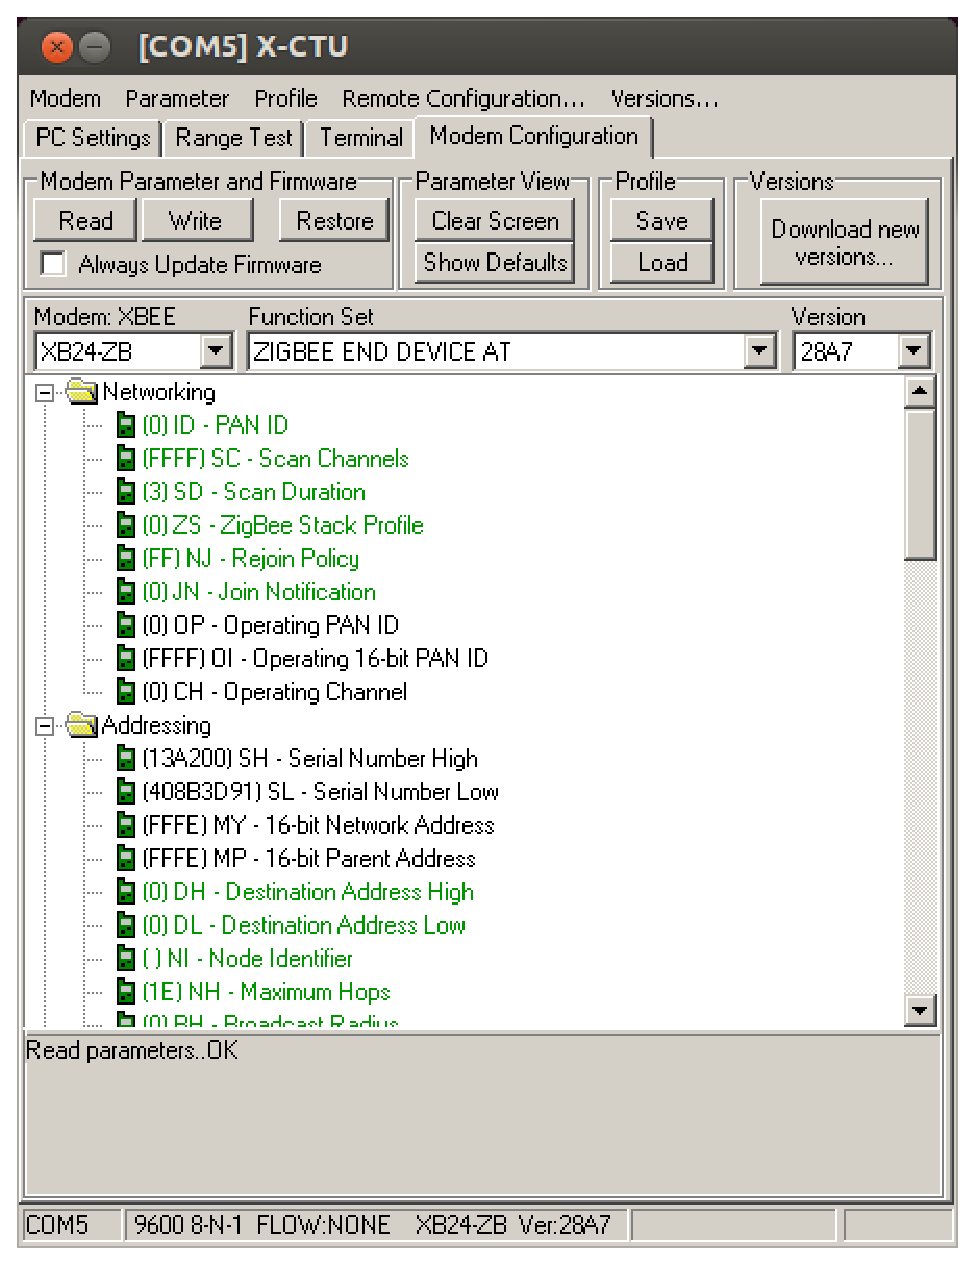
\includegraphics[width=0.3\linewidth]{figures/clean-28a7}
  \caption{Clean 28a7}
  \label{fig:clean-28a7}
\end{figure}

Let's prepare the new configuration.
Set the PAN ID to your group ID.
Set D0 to analog (2).
Set the sampling rate to 255 ms (IR=1FF).
We write the changes to the XBee.
The configuration should look as shown in Fig. \ref{fig:configured-end-device}

\begin{figure}[htbp]
  \centering
  \includegraphics[width=0.3\linewidth]{figures/configured-end-device}
  \caption{Configured end device. D0 set to 2 and IR set to 1FF.}
  \label{fig:configured-end-device}
\end{figure}

Now we need to configure the coordinator just as we configured it for 
Chapter \ref{cha:sink-in-server}.
We write a coordinator API firmware and restore to factory defaults.

We set the PAN ID.
And we write the configuration.

Now run the python program to read incoming data, and we will see as our screens fills with the received data, as in Fig. \ref{fig:received-data}.

\begin{figure}[htbp]
  \centering
  \includegraphics[width=0.3\linewidth]{figures/received-data}
  \caption{Data received by the XBee connected to the computer.}
  \label{fig:received-data}
\end{figure}

We have not sleep much so far.
It's time for a nap.
In the end device, change the ATSM to 5.
This gives us the possibility of waking up the XBee using the DTR pin.
Now we change the SP to 200 (default is 20) and we will see that the XBee takes a nap, then sends a few samples, and then takes a nap again.
Let's set the SP to AAA so that the naps are longer.
You will observe that the naps are fairly long, so we can use the DTR pin to wake the XBee.
We can also wake up the XBee for a round of measures by changing the DTR pin from high to low.

Repeat the lab assignment ``collecting data in a computer'' but this time the sensors will be awake for 1 second and then sleep for 10 seconds.
While the sensor is awake, it will send a sample every 100ms.

Now we will connect an LED between DIO9 and ground to see when the XBee wakes up.
Other ways to know when the XBee wakes up are looking at the RSSI led or the CTS flag in the ``terminal'' tab in X-CTU.

Now for a really long sleeping time, set the sleep options (SO) to 4.
This tells the XBee that, in case of not receiving any packets, it should multiply the sleep time by the value in SN (number of sleep periods).
Set SN also to 4 and save the settings to multiply by 4 the sleep time.

\section{Next Steps}
We can try sleeping in an actuator network.
In this case, we have to set the SP to the parent equal to the longest SP of all the children, to make sure that the parent stores the packets until the children wake up.
